\documentclass[tikz,border=4pt]{standalone}
\usepackage{libertine}
\usetikzlibrary{arrows.meta,calc,positioning,fit,backgrounds,shapes.geometric}
\definecolor{paperink}{HTML}{263441}
\definecolor{papermuted}{HTML}{647481}
\definecolor{paperline}{HTML}{CCD5DB}
\definecolor{paperblue}{HTML}{2D5F91}
\definecolor{paperbluefill}{HTML}{EFF5FA}
\definecolor{paperorange}{HTML}{B66731}
\definecolor{paperorangefill}{HTML}{FCF4EB}
\definecolor{papergreen}{HTML}{3F7558}
\definecolor{papergreenfill}{HTML}{EFF6F1}
\tikzset{
  papertext/.style={font=\footnotesize, text=paperink},
  papermini/.style={font=\scriptsize, text=papermuted},
  paneltitle/.style={font=\footnotesize\bfseries, text=paperink},
  bluebox/.style={draw=paperblue, fill=paperbluefill, rounded corners=1pt,
    line width=.6pt, font=\footnotesize, text=paperink, align=center,
    inner xsep=6pt, inner ysep=5pt},
  orangebox/.style={draw=paperorange, fill=paperorangefill, rounded corners=1pt,
    line width=.6pt, font=\footnotesize, text=paperink, align=center,
    inner xsep=6pt, inner ysep=5pt},
  greenbox/.style={draw=papergreen, fill=papergreenfill, rounded corners=1pt,
    line width=.6pt, font=\footnotesize, text=paperink, align=center,
    inner xsep=6pt, inner ysep=5pt},
  graybox/.style={draw=paperline, fill=white, rounded corners=1pt,
    line width=.6pt, font=\footnotesize, text=paperink, align=center,
    inner xsep=6pt, inner ysep=5pt},
  orangeflow/.style={-{Stealth[length=2mm]}, draw=paperorange, line width=1pt},
  blueflow/.style={-{Stealth[length=2mm]}, draw=paperblue, line width=1.15pt},
  greenflow/.style={-{Stealth[length=2mm]}, draw=papergreen, line width=1pt},
  grayflow/.style={-{Stealth[length=1.8mm]}, draw=papermuted, line width=.65pt}
}

\begin{document}
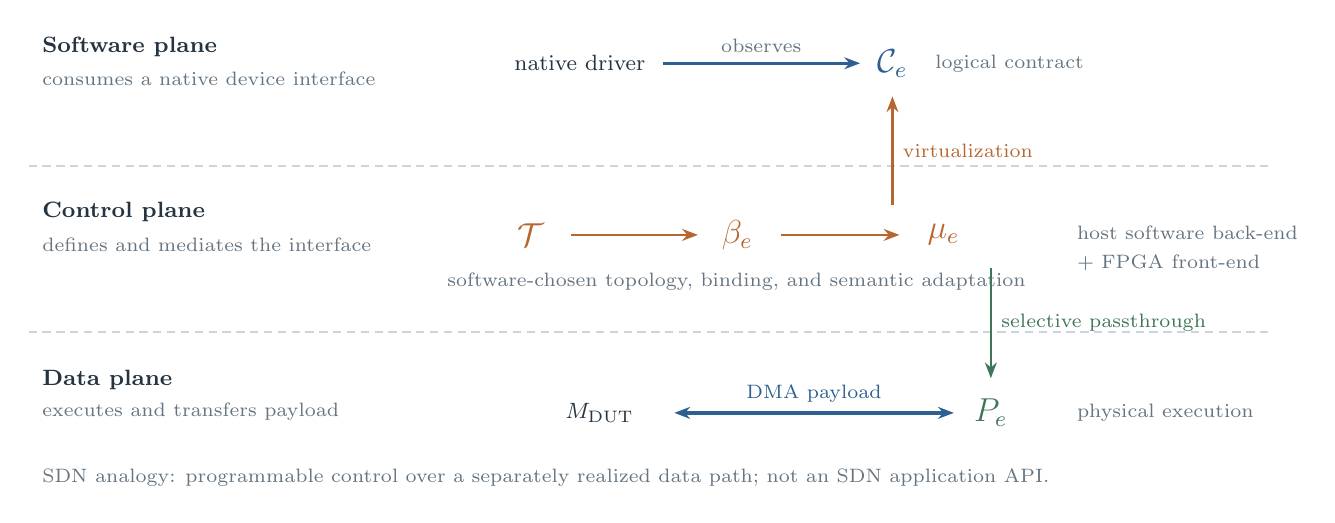
\begin{tikzpicture}[x=1cm,y=1cm]
  % Three functional planes. Geography is deliberately suppressed.
  \foreach \y in {2.21,4.32} {
    \draw[paperline, densely dashed, line width=.7pt] (.15,\y) -- (15.92,\y);
  }
  \node[paneltitle, anchor=west] at (.20,5.83) {Software plane};
  \node[papermini, anchor=west] at (.20,5.42) {consumes a native device interface};
  \node[paneltitle, anchor=west] at (.20,3.73) {Control plane};
  \node[papermini, anchor=west] at (.20,3.32) {defines and mediates the interface};
  \node[paneltitle, anchor=west] at (.20,1.60) {Data plane};
  \node[papermini, anchor=west] at (.20,1.19) {executes and transfers payload};

  \node[papertext] at (7.15,5.62) {native driver};
  \node[font=\large, text=paperblue] at (11.12,5.62) {$\mathcal{C}_e$};
  \draw[blueflow] (8.20,5.62) -- node[papermini, above] {observes} (10.71,5.62);
  \node[papermini, anchor=west] at (11.54,5.62) {logical contract};

  \node[font=\large, text=paperorange] at (6.53,3.44) {$\mathcal{T}$};
  \node[font=\large, text=paperorange] at (9.15,3.44) {$\beta_e$};
  \node[font=\large, text=paperorange] at (11.77,3.44) {$\mu_e$};
  \draw[orangeflow] (7.04,3.44) -- (8.65,3.44);
  \draw[orangeflow] (9.70,3.44) -- (11.21,3.44);
  \node[papermini] at (9.14,2.85)
    {software-chosen topology, binding, and semantic adaptation};
  \node[papermini, anchor=west] at (13.34,3.47) {host software back-end};
  \node[papermini, anchor=west] at (13.34,3.08) {+ FPGA front-end};

  \node[papertext] at (7.40,1.18) {$M_{\mathrm{DUT}}$};
  \node[font=\large, text=papergreen] at (12.37,1.18) {$P_e$};
  \draw[paperblue, line width=1.3pt, {Stealth[length=2mm]}-{Stealth[length=2mm]}]
    (8.35,1.18) -- node[papermini, above, text=paperblue] {DMA payload} (11.90,1.18);
  \node[papermini, anchor=west] at (13.34,1.18) {physical execution};

  \draw[paperorange, line width=.95pt, -{Stealth[length=2mm]}]
    (11.12,3.82) -- node[papermini, right, text=paperorange]
    {virtualization} (11.12,5.20);
  \draw[papergreen, line width=.95pt, -{Stealth[length=2mm]}]
    (12.37,3.02) -- node[papermini, right, text=papergreen]
    {selective passthrough} (12.37,1.62);
  \node[papermini, anchor=west] at (.20,.36)
    {SDN analogy: programmable control over a separately realized data path; not an SDN application API.};
\end{tikzpicture}
\end{document}
